\section{Supplementary Sensitivity Analysis}
\label{app:sensitivity_analysis}

This appendix provides extended sensitivity analyses for both Judge (RQ1a) and Corrector (RQ1b) prompts, quantifying performance stability across prompt variations.

\subsection{Judge Prompt Sensitivity}
\label{app:judge_sensitivity}

To quantify how prompt engineering choices affect judge performance, we perform a sensitivity analysis measuring the relationship between prompt variation (input) and F1 change (output). For judge prompts (RQ1a), prompt distances are computed as cosine distance from the baseline prompt using MPNet embeddings. We use \textbf{repeated-measures ANOVA} with CLD$\times$run as subjects and prompt as the within-subject factor, reporting \textbf{partial $\eta^2$} as the effect size (proportion of within-subject variance explained by prompt). Bonferroni correction is applied across the four RQ1a tests ($\alpha_{\text{adj}} = 0.0125$).

\subsubsection{Derivation: First-Order Sobol Index for a Categorical Factor}
\label{app:sobol_eta2_derivation}

For a single categorical factor $A \in \{1,\dots,K\}$ with $p_a = \Pr(A=a)$, define $\mu_a := \mathbb{E}[Y \mid A=a]$ and $\mu := \mathbb{E}[Y] = \sum_{a=1}^K p_a \mu_a$. The first-order Sobol index for $A$ is:
\begin{equation}
S_A := \frac{\mathrm{Var}(\mathbb{E}[Y \mid A])}{\mathrm{Var}(Y)}.
\end{equation}
Since $\mathbb{E}[Y \mid A]$ takes value $\mu_a$ when $A=a$, we have
\begin{equation}
\mathrm{Var}(\mathbb{E}[Y \mid A]) = \sum_{a=1}^K p_a(\mu_a - \mu)^2.
\end{equation}
By the law of total variance,
\begin{equation}
\mathrm{Var}(Y) = \mathbb{E}[\mathrm{Var}(Y \mid A)] + \mathrm{Var}(\mathbb{E}[Y \mid A])
= \sum_{a=1}^K p_a\,\mathrm{Var}(Y \mid A=a) + \sum_{a=1}^K p_a(\mu_a - \mu)^2.
\end{equation}
Hence,
\begin{equation}
S_A = \frac{\sum_{a=1}^K p_a(\mu_a - \mu)^2}{\mathrm{Var}(Y)} = \eta^2,
\end{equation}
i.e., the population one-way ANOVA effect size (correlation ratio) for a categorical factor~\cite{saltelli2010variance}. In the main experiments, we report $\eta^2_p$ (partial eta-squared) because our design is blocked by CLD$\times$run (repeated measures), so the sensitivity measure is computed after controlling for these subject-level differences.

\begin{figure}[H]
\centering
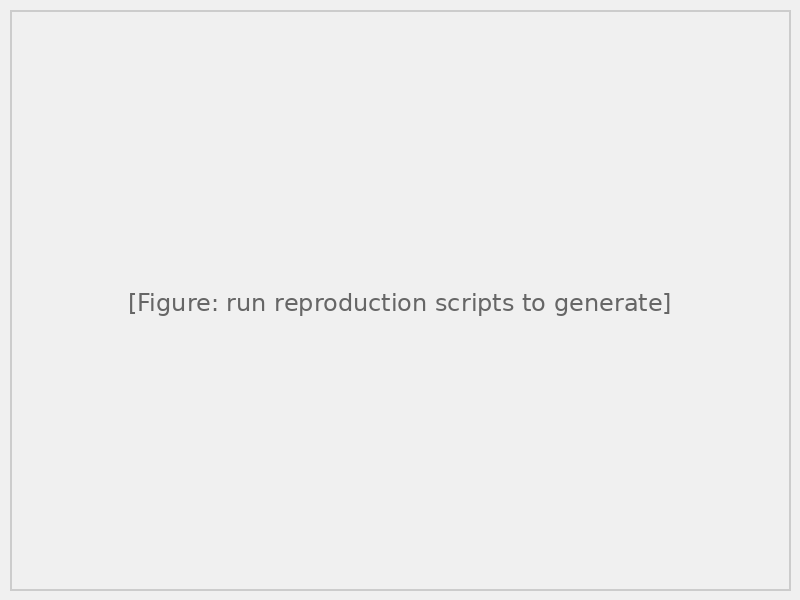
\includegraphics[width=1.0\textwidth]{../../final_runs/Sensitivity_analysis_simple/prompt_sensitivity_figure.png}
\caption{Prompt sensitivity analysis across RQ1a experiments. Each panel shows F1 performance (mean $\pm$ std across CLDs and runs) for prompt variants. Statistical test: repeated-measures ANOVA with partial $\eta^2$; significance indicated by * $p<0.05$, ** $p<0.01$, *** $p<0.001$; $\dagger$ significant after Bonferroni correction. Dashed lines indicate baseline.}
\label{fig:sensitivity_analysis_app}
\end{figure}

Figure~\ref{fig:sensitivity_analysis_app} shows that prompt effects are strongest for the correctness judge (Corruption Detection: $\eta^2_p=0.62$, $p<0.001$; Ground Truth: $\eta^2_p=0.68$, $p<0.001$), with large effect sizes indicating that 62--68\% of within-subject variance is explained by prompt choice. Citation judge effects are weaker (Corruption Detection: $\eta^2_p=0.31$, $p=0.030$) and do not survive Bonferroni correction.

\begin{table}[H]
\centering
\footnotesize
\caption{Judge Prompt Sensitivity Analysis}
\label{tab:prompt_sensitivity}
\begin{threeparttable}
\resizebox{\textwidth}{!}{%
\begin{tabular}{@{}llccccccc@{}}
\toprule
\textbf{Experiment} & \textbf{Prompt} & \textbf{Dist.} & \textbf{F1} & \textbf{Std} & \textbf{95\% CI} & \textbf{$\Delta$F1} & \textbf{$\eta^2_p$} & \textbf{p} \\
\midrule
Corr. Cit. & Baseline & 0.00 & 0.397 & 0.038 & [0.366, 0.428] & +0.000 & \multirow{4}{*}{0.31} & \multirow{4}{*}{0.122} \\
 & CoT & 0.02 & 0.398 & 0.038 & [0.367, 0.429] & +0.001 &  &  \\
 & Mechanistic & 0.32 & 0.400 & 0.037 & [0.370, 0.430] & +0.003 &  &  \\
 & Mech-Lit & 0.31 & 0.401 & 0.038 & [0.370, 0.431] & +0.004 &  &  \\
\midrule
Corr. Corr. & Baseline & 0.00 & 0.764 & 0.049 & [0.724, 0.804] & +0.000 & \multirow{3}{*}{0.59} & \multirow{3}{*}{0.003**} \\
 & CoT & 0.01 & 0.776 & 0.050 & [0.735, 0.816] & +0.012 &  &  \\
 & Mechanistic & 0.18 & 0.717 & 0.042 & [0.683, 0.751] & -0.047 &  &  \\
\midrule
GT Cit. & Baseline & 0.00 & 0.299 & 0.083 & [0.231, 0.366] & +0.000 & \multirow{4}{*}{0.43} & \multirow{4}{*}{0.012*} \\
 & CoT & 0.02 & 0.297 & 0.089 & [0.225, 0.370] & -0.001 &  &  \\
 & Mechanistic & 0.32 & 0.280 & 0.076 & [0.218, 0.342] & -0.019 &  &  \\
 & Mech-Lit & 0.31 & 0.267 & 0.074 & [0.206, 0.327] & -0.032 &  &  \\
\midrule
GT Corr. & Baseline & 0.00 & 0.206 & 0.076 & [0.144, 0.268] & +0.000 & \multirow{3}{*}{0.68} & \multirow{3}{*}{$<$.001***} \\
 & CoT & 0.01 & 0.235 & 0.063 & [0.183, 0.286] & +0.029 &  &  \\
 & Mechanistic & 0.18 & 0.447 & 0.120 & [0.349, 0.545] & +0.241 &  &  \\
\bottomrule
\end{tabular}
}%
\begin{tablenotes}
\scriptsize
\item \textit{Note.} Dist. = MPNet cosine distance from baseline. $\eta^2_p$ = partial eta-squared (RM-ANOVA). N=9 per prompt.
\item 95\% CI computed using t-distribution ($df=8$) for block-level meta-inference per uncertainty reporting rule.
\item p-values are Bonferroni-corrected (4 tests, $\alpha_{adj}$=0.0125). * $p<.05$, ** $p<.01$, *** $p<.001$.
\end{tablenotes}
\end{threeparttable}
\end{table}

\begin{table}[H]
\centering
\caption{RM-ANOVA Assumption Checks for Judge Prompt Sensitivity (Appendix K)}
\label{tab:prompt_sensitivity_assumptions}
\begin{threeparttable}
\scriptsize
\setlength{\tabcolsep}{3pt}
\renewcommand{\arraystretch}{1.1}
\begin{tabular}{lccccccl}
\toprule
\textbf{Exp.} & \textbf{$n$} & \textbf{$k$} & \textbf{Shapiro $p$} & \textbf{Mauchly $p$} & \textbf{$\epsilon_{GG}$} & \textbf{$p$ (unc.)} & \textbf{$p$ (GG)} \\
\midrule
Corr.\ Cit. & 9 & 4 & 0.002 & $<$.001 & 0.57 & 0.030 & 0.064 \\
Corr.\ Corr. & 9 & 3 & 0.429 & $<$.001 & 0.82 & $<$.001 & 0.002 \\
GT\ Cit. & 9 & 4 & 0.696 & $<$.001 & 0.49 & 0.003 & 0.021 \\
GT\ Corr. & 9 & 3 & 0.509 & $<$.001 & 0.57 & $<$.001 & 0.002 \\
\bottomrule
\end{tabular}
\begin{tablenotes}
\scriptsize
\item \textit{Note.} Shapiro-Wilk is applied to RM-ANOVA residuals (subject + prompt additive model). Mauchly's test assesses sphericity of the within-subject covariance. $\epsilon_{GG}$ is Greenhouse--Geisser epsilon; $p$ (GG) uses $\epsilon_{GG}$-adjusted degrees of freedom. For $k=2$, sphericity is not defined and Mauchly/GG are omitted.
\end{tablenotes}
\end{threeparttable}
\end{table}

Table~\ref{tab:prompt_sensitivity} shows that prompt choice significantly affects the correctness judge (large effects, $\eta^2_p>0.60$), while citation-judge prompt effects are moderate ($\eta^2_p\approx0.30$--0.43) with the corruption detection effect not surviving family-wise correction.

\subsection{Corrector Prompt Sensitivity}
\label{app:corrector_sensitivity}

Extending the sensitivity analysis to the LLM-as-a-Corrector (RQ1b), we evaluate how corrector prompt complexity affects correction performance. Unlike judge prompts which had distinct semantic content, corrector prompts follow a cumulative design: Baseline provides examples only, CoT adds step-by-step reasoning (1.45$\times$ length), and Mechanistic adds Bradford Hill criteria (1.91$\times$ length).
Because these prompts are long and share a common prefix, we compute corrector prompt distances using long-context Jina embeddings v2 (to avoid truncation artifacts in short-context encoders).

\begin{figure}[H]
\centering
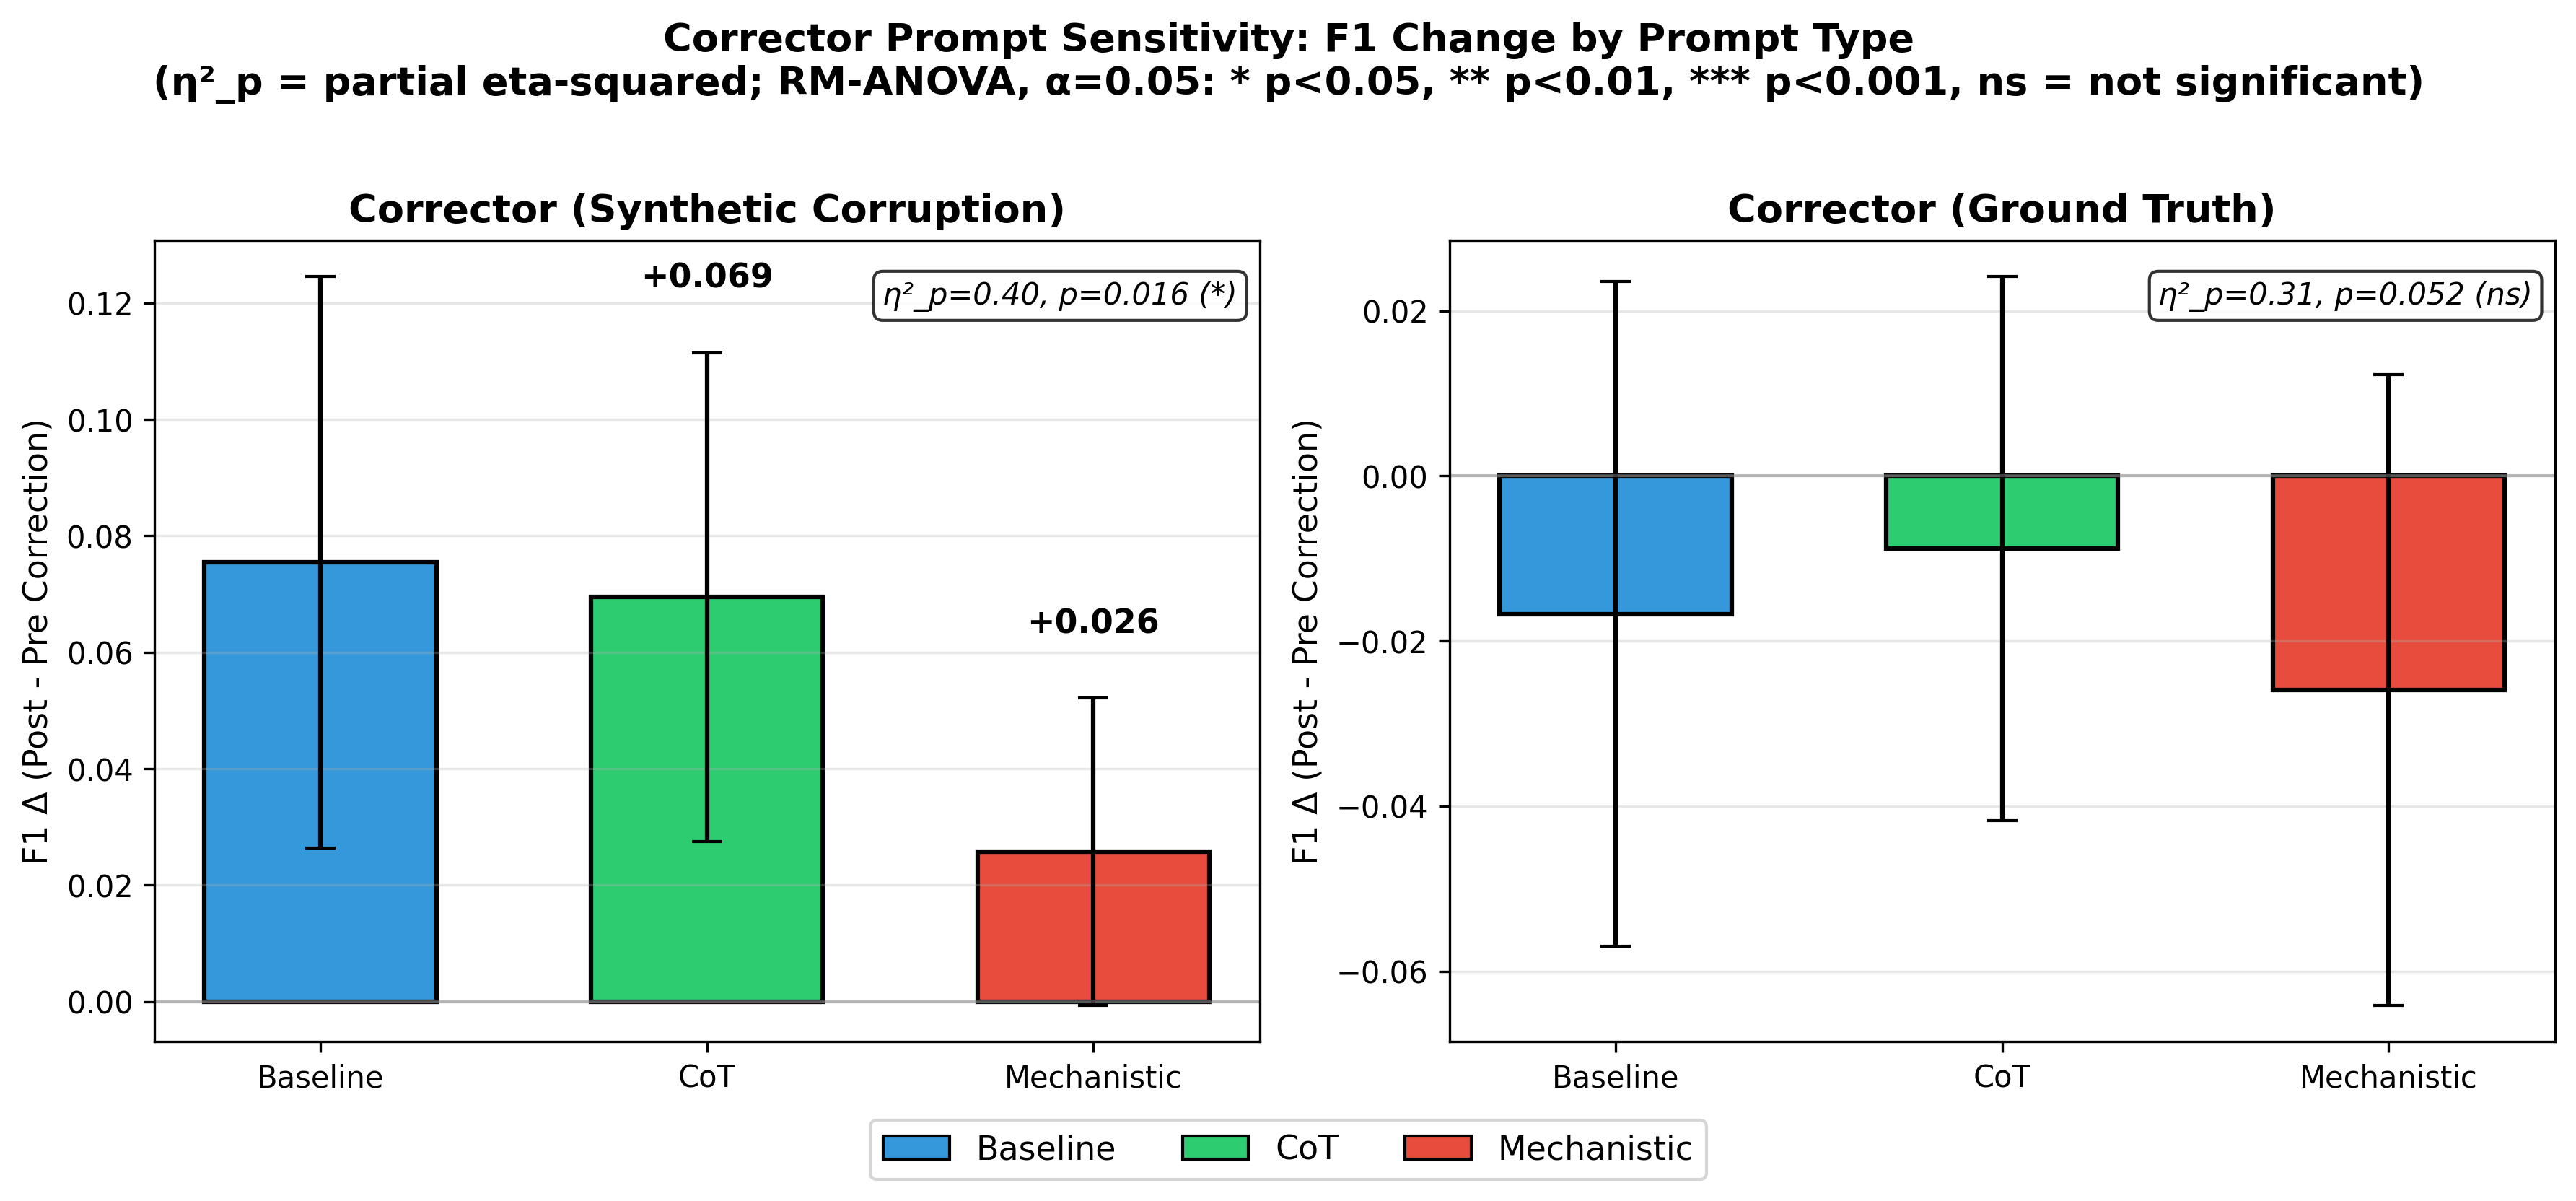
\includegraphics[width=1.0\textwidth]{../../final_runs/Sensitivity_analysis_simple/corrector_sensitivity_figure.png}
\caption{Corrector prompt sensitivity analysis. F1 $\Delta$ (post-correction minus pre-correction) by prompt type. Statistical test: repeated-measures ANOVA with partial $\eta^2$; significance: * $p<0.05$, ** $p<0.01$, *** $p<0.001$. Error bars show standard deviation across CLDs and runs.}
\label{fig:corrector_sensitivity_app}
\end{figure}

Figure~\ref{fig:corrector_sensitivity_app} shows a significant prompt effect for synthetic corruptions ($\eta^2_p=0.40$, $F(2,16)=5.43$, $p=0.016$), indicating that simpler prompts (Baseline: $+0.075$) outperform complex prompts (Mechanistic: $+0.026$). Ground truth correction shows a marginally significant effect ($\eta^2_p=0.31$, $p=0.052$).

\begin{table}[H]
\centering
\footnotesize
\caption{Corrector Prompt Sensitivity Analysis}
\label{tab:corrector_sensitivity}
\begin{threeparttable}
\begin{tabular}{@{}llccccccc@{}}
\toprule
\textbf{Experiment} & \textbf{Prompt} & \textbf{Dist.} & \textbf{F1$\Delta$} & \textbf{Std} & \textbf{95\% CI} & \textbf{Actions} & \textbf{$\eta^2_p$} & \textbf{p} \\
\midrule
Synth. & Baseline & 0.00 & +0.08 & 0.06 & [+0.03, +0.12] & 1006 & \multirow{3}{*}{0.40} & \multirow{3}{*}{0.032*} \\
 & CoT & 0.01 & +0.07 & 0.05 & [+0.03, +0.11] & 1006 &  &  \\
 & Mechanistic & 0.03 & +0.03 & 0.03 & [-0.00, +0.05] & 1006 &  &  \\
\midrule
GT & Baseline & 0.00 & -0.02 & 0.05 & [-0.06, +0.02] & 418 & \multirow{3}{*}{0.31} & \multirow{3}{*}{0.104} \\
 & CoT & 0.01 & -0.01 & 0.04 & [-0.04, +0.02] & 408 &  &  \\
 & Mechanistic & 0.03 & -0.03 & 0.05 & [-0.06, +0.01] & 418 &  &  \\
\bottomrule
\end{tabular}
\begin{tablenotes}
\scriptsize
\item \textit{Note.} Dist. = Jina v2 cosine distance from baseline. $\eta^2_p$ = partial eta-squared (RM-ANOVA). N=9 per prompt.
\item 95\% CI computed using t-distribution ($df=8$) for block-level meta-inference per uncertainty reporting rule.
\item p-values are Bonferroni-corrected (2 tests, $\alpha_{adj}$=0.025). * $p<.05$, ** $p<.01$, *** $p<.001$.
\end{tablenotes}
\end{threeparttable}
\end{table}

\begin{table}[H]
\centering
\caption{RM-ANOVA Assumption Checks for Corrector Prompt Sensitivity (Appendix K)}
\label{tab:corrector_sensitivity_assumptions}
\begin{threeparttable}
\scriptsize
\setlength{\tabcolsep}{3pt}
\renewcommand{\arraystretch}{1.1}
\begin{tabular}{lccccccl}
\toprule
\textbf{Exp.} & \textbf{$n$} & \textbf{$k$} & \textbf{Shapiro $p$} & \textbf{Mauchly $p$} & \textbf{$\epsilon_{GG}$} & \textbf{$p$ (unc.)} & \textbf{$p$ (GG)} \\
\midrule
Synth. & 9 & 3 & 0.516 & $<$.001 & 0.54 & 0.016 & 0.044 \\
GT Lit & 9 & 3 & 0.119 & $<$.001 & 0.72 & 0.052 & 0.073 \\
\bottomrule
\end{tabular}
\begin{tablenotes}
\scriptsize
\item \textit{Note.} Shapiro-Wilk is applied to RM-ANOVA residuals (subject + prompt additive model). Mauchly's test assesses sphericity of the within-subject covariance. $\epsilon_{GG}$ is Greenhouse--Geisser epsilon; $p$ (GG) uses $\epsilon_{GG}$-adjusted degrees of freedom. For $k=2$, sphericity is not defined and Mauchly/GG are omitted.
\end{tablenotes}
\end{threeparttable}
\end{table}

The table above summarizes the repeated-measures ANOVA results for corrector prompt sensitivity.

